\documentclass[a4paper,1  pt]{report}
\usepackage[utf8]{inputenc}
\usepackage[ LAE ]{fontenc}
\usepackage[farsi,english,arabic]{babel}
\usepackage{graphicx}
\usepackage{float}
\graphicspath{{./images/}}

\title{\textRL{الملاحقة بالاعتماد على تقنيات التعلم العميق}}
\author{مي عبود}

\begin{document}

\maketitle
\tableofcontents
%\begin{abstract}
%\end{abstract}


\chapter{المقدمة}
\section{المصطلحات والتعاريف}
 
\subsubsection{\textLR{Visual object tracking}}

\subsubsection{\textLR{short-term tracking}}
 هدفها تقدير حالة الغرض حتى تفشل عملية الملاحقة.
\subsubsection{\textLR{model-based trackers}}
  هي الملاحقات التي تلاحق صنف واحد من الأغراض.
\subsubsection{\textLR{model-free trackers}}
هي الملاحقات التي تلاحق أغراض عامة وذلك بتحديد الغرض في أول إطار للفيديو.
\subsubsection{\textLR{self-attention}}
تنتج عن حساب الجداء الداخلي لمصفوفتي
\textLR{query and key matrix}

\subsubsection{\textLR{AO: average overlap}}
وهو مقياس لمقارنة أداء خوارزميات الملاحقة معتمد في مجموعة المعطيات
\textLR{got10k}
التي نتعامل معها في مشروعنا. و هي عبارة عن الوسطي للـ
\textLR{IOU}
بين الـ 
\textLR{groundtruth}
وبين نتيجة الملاحق.
\subsubsection{\textLR{IOU : intersection over union}}
ضع معادلة 
\textLR{IOU}
 بالإضافة إلى رسمة توضيحية.
\subsubsection{\textLR{SR(ratio)}}
أيضا هو معيار مستخدم من قبل مجموعة المعطيات الخاصة بالملاحقة للمقارنة بين أداء الخوارزميات ،ويعبر عن نسبة الصور  التي يكون 
\textLR{IOU}
أكبر من قيمة 
\textLR{ratio}.
\newline\newline
\subsection{تعريف الملاحقة}
تعرف الملاحقة بأنها تقدير لحالة الغرض المراد ملاحقته في الصور المتلاحقة للفيديو  بالاعتماد فقط على مظهر الهدف في الإطار الأول. معظم خوارزميات الملاحقة لغرض واحد تكتفي بتقدير مكان لغرض ومستطيل محيط به، ويتم يدويا تحديد هذا المستطيل في الإطار الأول لعملية الملاحقة. 
\newline
أو تعريف اخر .
تعريف الملاحقة
\textLR{\cite{Zhao21}}
 هي مهمة تقدير حالة الغرض المراد ملاحقته في أطر الفيديو المتلاحقة. حالة الغرض يمكن التعبير عنها بمستطيل محيط بالغرض في كل إطار في الفيديو ندعوه
\textLR{bounding box}.
في الإطار الأول من الصورة يعطى المستطيل الابتدائي، والمهمة هي تقدير المستطيلات المحيطة بالهدف في الأطر المتتالية.
\newline
يمكن وضع صورة هنا توضح عملية اختيار الهدف في الإطار الأول، وصورة ثاتية تعبر عن نتيجة الملاحقة.
يمكن وضع مشكلات البحث هنا .....

 وكما هو الحال في مجالات الرؤية الصنعية الأخرى كالكشف والتعرف و… فإن تقنيات تعلم الالة وخاصة التعلم العميق هي المسيطرة في الوقت الحالي على الخوارزميات وذلك بسبب توفر معطيات تدريب كبيرة، فأصبحت عملية استخلاص السمات من خلال الشبكات العميقة أكثر فعالية من الطرق التقليدية، وأصبح من الممكن تدريب خوارزميات ذات طبقات عميقة.  من أهم هذه الأبحاث نذكر
\textLR{siamFC,OCEAN,}
 من التقنيات الحديثة في التعلم العميق والتي أعطت أداء فعال هي المحول
\textLR{transformer}
 وقد ظهرت في عام
\textLR{2017}
 ليستخدم في تطبيقات معالجة اللغات الطبيعي، كما أنها أيضا أعطت أداء فعال في تطبيقات الرؤية الحاسوبية.
 في سنة
\textLR{2021}
 ظهرت عدة خوارزميات ملاحقة استفادت من تقنية المحول، نذكر منها خوارزمية 
\textLR{STARK، swintrack , transtrack }
أعطت هذه الخوارزميات نتائج متفوقة على الخوارزميات السابقة وقت ظهورها.

إحدى المشكلات الأساسية في معظم الخوارزميات المذكورة سابقا، هي اعتمادها فقط على المعلومات المكانية لتحديد الهدف، نقصد بالمعلومات المكانية هي المنطقة المحيطة بالهدف
\textLR{search window}.
في خوارزمية
\textLR{STARK}
هناك محاولة للاستفادة من المعلومات الزمنية وذلك بإضافة دخل جديد وهو
\textLR{updated template}
إلى الشبكة.
من النقاط الأساسية التي يعالجها هذا البحث هو الاستفادة من المعلومات الزمانية 
\textLR{temporal information}
الناتجة عن تسلسل الصور . إذ تفتقر العديد من خوارزميات الملاحقة لمعالجة هذا النوع من المعطيات وتكتفي بالمعلومات المكانية
\textLR{spatial information}
كخوارزميات الملاحقة عن طريق الكشف.
\newline{}
من المساهمات الأساسية لهذا البحث هي الاستفادة من المعلومات الزمانية كما في خوارزمية 
\textLR{stark}
وذلك عن طريق استخدم
\textLR{update template}
ولكن بطريقة مختلفة عنها، إذ في خوارزمية
\textLR{stark}
يتم دمج السمات للـ
\textLR{template}
المبدئي المأخوذ من الصورة الأولى وسمات الـ 
\textLR{updated template ، }
عن طريق
\textLR{concatenation }
في بحثنا تم تجريب دمج شعاعي السمات عن طريق استخدام
\textLR{multihead attention ،}
وهي البنية الأساسية في خوارزمية
\textLR{transformer. }
وقد أعطت هذه الطريقة نتائج جيدة، وزمن تدريب أقل إذ لاحاجة لتغيير أبعاد بنية الـ 
\textLR{encoder}
إذ تضمن عملية دمج السمات عن طريق 
\textLR{multihead attention }
المحافظة على أبعاد البنية الأساسية للخوارزمية ، وبالتالي الاستفادة من البارامترات المدربة مسبقا.
في بحثنا تم الاعتماد على تحسين خوارزمية 
\textLR{swintrack ،}
كونها لا تستخدم المعلومات الزمنية
\section{مشكلة البحث}
يتم تقييم خوارزمية الملاحقة من خلال قدرتها على تتبع الهدف الملاحَق وتجاوز التغيرات التي يعاني منها الهدف أو البيئة المحيطة بالهدف. وسنتوسع في هذه الفقرة بالتحديات التي تواجه الملاحقة كما ذكرها المرجع
\cite{Abbass21}
\begin{itemize}
  \item
   تغير شكل الغرض إما بسبب تغير زاوية الرؤية، أو بسبب طبيعة الجسم المفصلية.
  \item
  يمكن أن تكون الملاحقة ضمن بيئة عالية الديناميكية، حيث أن كل من الكاميرا والهدف في حالة حركة، وهذا ما يعقد عملية تحليل والتنبؤ بالحركة.
  \item
  الملاحقة بالزمن الحقيقي، إذ تتطلب بعض التطبيقات أن يكون الملاحق ذو أداء عالي و في نفس الوقت قادر على معالجة الصور المتلاحقة الزمن الحقيقي.
  \item
  تغيير الإضاءة.
  \item
  وجود أغراض مشابهة للغرض المراد ملاحقته، أو وجود خلفية لها نفس بنية الغرض، وهذا ما يجعل الغرض يتماهى مع الخلفية، وبالتالي تزداد صعوبة الملاحقة.
  \item
  دقة الكاميرا المستخدمة.
  \item
  احتجاب الغرض  جزئيا أو كليا.
  \item
  اختفاء الغرض كليا من المشهد.
  \item
  الحركات المفاجئة للغرض
\end{itemize}

\section{المساهمات األساسية للبحث}
\section{بنية الأطروحة}
تتضمن الأطروحة
\section{مجموعة المعطيات}

\selectlanguage{english}
\begin{figure}[H]
    \centering
    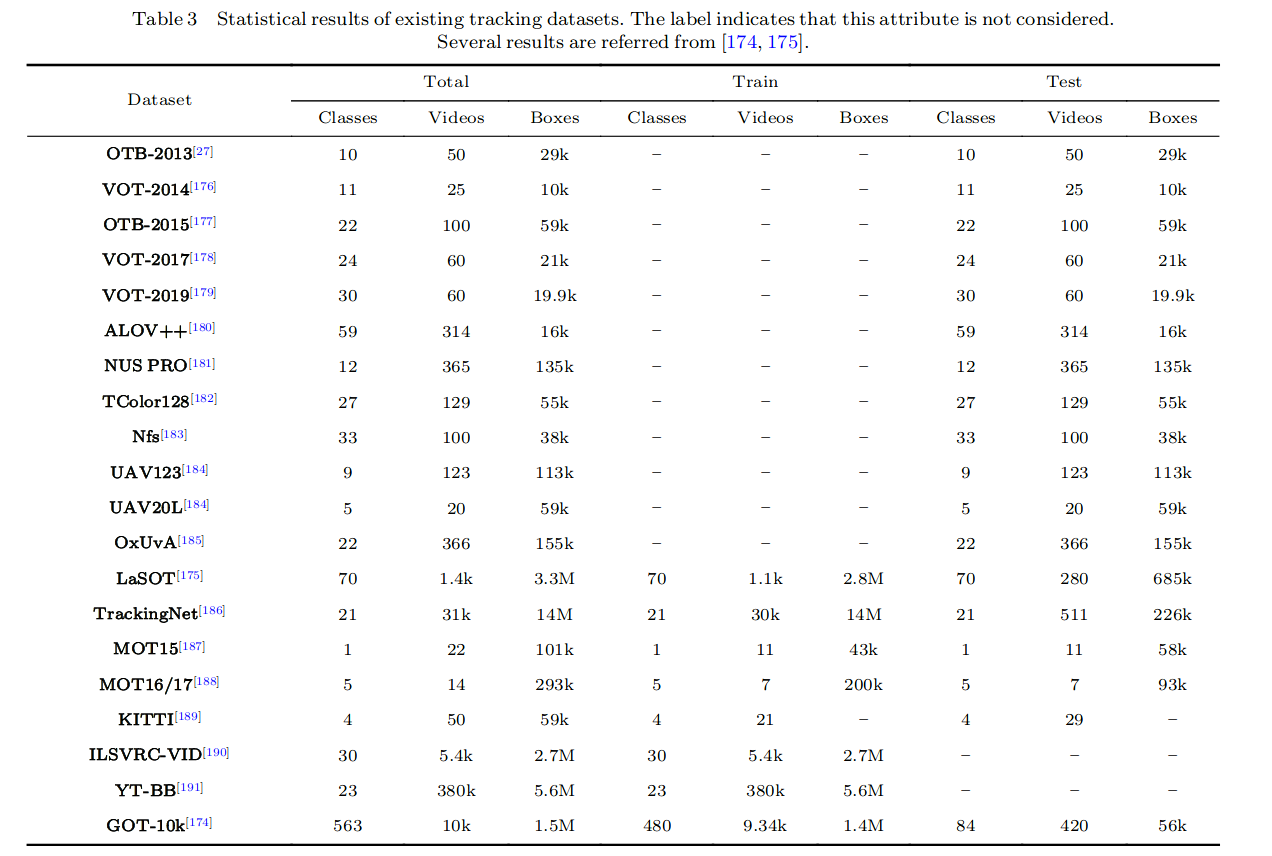
\includegraphics[width=\textwidth]{images/table_dataset}
    \caption{\textRL{مجموعات المعطيات الخاصة بمسألة الملاحقة}\cite{Zhang21}}
\end{figure}
\selectlanguage{arabic}
أهم مجموعات المعطيات الخاصة بمسألة الملاحقة لغرض واحد هي 
\textLR{Got10k, LaSot, TrackingNet, VOT, OTB}
هذه المجموعات يمكن أن ندرب أو نختبر الخوارزميات بواسطتها
اخترنا تدريب النموذج على مجموعو المعطيات
\textLR{Got10k}
كونها الأقل حجما ( هنا اذكري الحجم)، ولكن هي الأكثر تنوعا بين مجموعات المعطيات الأخرى
\section{تقييم الأداء}
لكل مجموعة معطيات سابقة معاييرها الخاصة للمقارنة بين أداء الملاحقات :
نذكر من هذه المعايير :
\begin{itemize}
  \item \textLR{Precision}
  \item \textLR{Success and accuracy}
  \item \textLR{Robustness}
  \item \textLR{AO}
  
  
\end{itemize}

\section{توابع الخطأ}

\section{تصنيف الملاحقات}

\selectlanguage{english}
\begin{thebibliography}{ widest-label }
\bibitem{Zhang21}
\label{Zhang et al., 2021}
Zhang, X.-Q., Jiang, R.-H., Fan, C.-X., Tong, T.-Y., Wang, T., Huang, P.-C., 2021. Advances in Deep Learning Methods for Visual Tracking: Literature Review and Fundamentals. International Journal of Automation and Computing 18, 311–333. https://doi.org/10.1007/s11633-020-1274-8
\bibitem{Abbass21}Abbass, M.Y., Kwon, K.-C., Kim, N., Abdelwahab, S.A., El-Samie, F.E.A., Khalaf, A.A.M., 2021. A survey on online learning for visual tracking. Vis Comput 37, 993–1014. https://doi.org/10.1007/s00371-020-01848-y
\bibitem{Zhao21}Zhao, M., Okada, K., Inaba, M., 2021. TrTr: Visual Tracking with Transformer. arXiv:2105.03817 [cs].

\end{thebibliography}
\end{document}
